\subsection{Caso de uso : } \label{cu}
\subsubsection{Resumen}
Este caso de uso le permite al actor poder desactivar su cuenta en cualquier momento dado.
\subsubsection{Descripción}
\begingroup
\setlength{\LTleft}{-10cm plus -1fill}
\setlength{\LTright}{\LTleft}
\begin{center}
  \captionof{table}{} \label{tab:cu_tab}
  \begin{longtable}{| p{3.5cm} | p{11.5cm} |}
        \hline
        \textbf{Versión} &  0.1 \\
        \hline 
        \textbf{Autor} & Juan Gerardo Diaz Rodarte \\
        \hline
          \textbf{Estatus} & Edición \\
        \hline  
          \textbf{Fecha de último estatus} & 3 de abril de 2017 \\
        \hline
      \multicolumn{2}{c |}{\large{Atributos:}} \\
        \hline
          \textbf{Actor} & Usuario y Sub-Usuario \\
        \hline  
          \textbf{Propósito} &  Desactivar la cuenta del actor en cualquier momento dado. \\
        \hline
          \textbf{Disparador} & El actor presiona el botón Btn Desactivar cuenta en la vista IU Editar perfil. \\
        \hline  
          \textbf{Entradas} & No hay entradas. \\
        \hline  
          \textbf{Salidas} & 
           \begin{itemize}
	   \item \textbf{\ref{msjn_09}}
	 \end{itemize}\\
        \hline  
          \textbf{Precondiciones} & 
	\begin{itemize}
	   \item \textbf{Interna:} El actor debe estar registrado en el sistema.
	   \item \textbf{Interna:} El actor debe haber iniciado sesión en el sistema.
	 \end{itemize} \\
        \hline  
          \textbf{Postcondiciones} & 
	\begin{itemize}
              \item \textbf{Interna:} La cuenta del usuario pasará a un estado de \textit{desactivada}.
	\end{itemize} \\
        \hline
          \textbf{Reglas de negocio} & \\
        \hline
          \textbf{Mensajes} & \\
        \hline
          \textbf{Tipo} & \\
        \hline      
  \end{longtable}
\end{center}
\endgroup

\subsubsection{Trayectorias del caso de uso}
\textbf{Trayectoria principal}
\begin{enumerate}
  \item {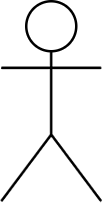
\includegraphics[scale=.1]{Capitulo3/img/actor.png} }
  \item {
\includegraphics[scale=.05]{Capitulo3/img/proceso.png}}
  \textit{Fin de caso de uso} \\  
\end{enumerate}

\textbf{Trayectoria alternativa} \phantomsection\label{cu_ta_} \\
\textbf{Condición:} \\
 \begin{enumerate}[label=\arabic*]
    \item {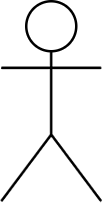
\includegraphics[scale=.1]{Capitulo3/img/actor.png} }
    \item {
\includegraphics[scale=.05]{Capitulo3/img/proceso.png}}
    \item {Continua en el paso 4 de la trayectoria principal.} \\
    \textit{Fin de trayectoria} \\
\end{enumerate}

\subsubsection{Puntos de extensión}
\noindent \textbf{Causa de la extensión:} \\
\textbf{Región de la trayectoria:} \hyperref[cu_ta_]{Trayectoria alternativa } \\
\textbf{Extiende a:} \hyperref[cu]{CU}
